\section{Comparison}\label{sec:comparison}

In this section, a comparison of the measurements performed on the different DUTs will be performed. This will be done in a manner where all test case measurements will be summed to a boxplot. When analyzing the results, this will be done by looking at each of \textbf{RQ2-4} one at a time. But first, some expectations.


\subsection{Expectations:} 

Based on what was seen in \cref{sec:iterations}, similar observations are expected. This will include a clamp with a high standard deviation compared to the different software measuring instruments, and cases where IPG and LHM measurements will appear similar. For RAPL, a low standard deviation is expected, in addition to lower measured energy consumption in most cases compared to the other measuring instruments. E3 measurements are expected to be somewhere between RAPL and the measurements by IPG and LHM.


\subsection{Results}

When presenting the results, this will be done based on BinaryTrees and Nbody, as these test cases illustrate the different tendencies in the different test cases. The results from the additional test cases can be found in \cref*{app:comparison,app:comparison_surfacebook,app:comparison_surfacepro4,app:comparison_workstation}. Before going into the different research questions, some overall observations can be made. This is first of all regarding the standard deviation of the different measuring instruments, as seen for BinaryTrees and Nbody in \cref*{fig:BinaryTrees_Cores_comparison_dynamic_energy_without_outliers_avg_watts,fig:Nbody_Cores_comparison_dynamic_energy_without_outliers_avg_watts} respectively. The standard deviation for the clamp can be observed to be very high, compared to the different software measuring instruments.


                            \begin{figure}
                                \centering
                                \begin{tikzpicture}[]
                                    \pgfplotsset{%
                                        width=.85\textwidth,
                                        height=.15\textheight
                                    }
                                    \begin{axis}[xlabel={Average energy consumption (Watts)}, title={Cores - BinaryTrees - Energy - without outliers}, ytick={},
                                    yticklabels={
                                        
                                        },
                                        xmin=0,xmax=20,
                                        ]
                                    
                                    \end{axis}
                                \end{tikzpicture}
                            \caption{A comparison of of Cores energy consumption for test case BinaryTrees for the Surface4Pro,  experiment \#2 (without outliers)} \label{fig:BinaryTrees_Cores_comparison_energy_without_outliers_Surface4Pro_avg_watts_exp2}
                            \end{figure}
                            

                \begin{figure}[H]
                    \centering
                    \begin{tikzpicture}
                        \pgfplotsset{%
                            width=1\textwidth,
                            height=0.4\textheight
                        }
                        \begin{axis}[
                            xlabel={Start battery level},
                            ylabel={Average dynamic energy (watt)},
                            ymin=0,ymax=20,
                        ]
                        
                            \addplot [mark=none, ultra thick, red]  coordinates {
                            (40, 0.006595684402444291)(45, 0.007295220674193181)(50, 0.007999659608910881)(55, 0.007202467971243639)(60, 0.007280865079495958)(65, 0.006858423509955077)(70, 0.008369444141141925)(75, 0.007144940647010992)(80, 0.004753236834232667)
                            };
                            \addlegendentry{Surface4Pro - IntelPowerGadget}
                            
                            \addplot [mark=none, ultra thick, blue]  coordinates {
                            (40, 0.002385328427460912)(45, 0.0017856511573015649)(50, 0.0025901992189954056)(55, 0.00210998144366709)(60, 0.00286452646862575)(65, 0.0020038487280194628)(70, 0.002908483770774353)(75, 0.0005098111150931342)(80, -0.005995916826693459)
                            };
                            \addlegendentry{Surface4Pro - HardwareMonitor}
                            
                            \addplot [mark=none, ultra thick, orange]  coordinates {
                            (50, 251.8661014299577)(55, 214.7597259251014)(60, 162.23880995564176)(65, 107.43421593849766)(70, 53.9187387386668)(75, 0.7554852536149699)(80, -44.463085003568885)
                            };
                            \addlegendentry{Surface4Pro - RAPL}
                            
                            \addplot [mark=none, dashdotted, red]  coordinates {
                            (40, -0.004038062354887025)(45, -0.004312668500277529)(50, -0.003808663911021498)(55, -0.0037057407527755254)(60, -0.004478257932982471)(65, -0.0026308734995501644)(70, -0.0034090674446925874)(75, -0.003041497079697436)(80, -0.0020334307266356875)
                            };
                            \addlegendentry{SurfaceBook - IntelPowerGadget}
                            
                            \addplot [mark=none, dashdotted, blue]  coordinates {
                            (40, -0.002443518930616523)(45, -0.0029256880137447055)(50, -0.002551777773312929)(55, -0.0027567211782433486)(60, -0.002206859154402231)(65, -0.0026388300848279207)(70, -0.0024597736945479324)(75, -0.002445350799195827)(80, -0.000541271265011134)
                            };
                            \addlegendentry{SurfaceBook - HardwareMonitor}
                            
                            \addplot [mark=none, dashdotted, orange]  coordinates {
                            (40, 101.92702155010147)(45, 86.7212700795567)(50, 69.40754598562454)(55, 51.343785407669614)(60, 32.443112755251185)(65, 14.52577919077786)(70, -4.520517378551423)(75, -23.811706977384954)(80, -35.700372165212755)
                            };
                            \addlegendentry{SurfaceBook - RAPL}
                            
                        \end{axis}
                    \end{tikzpicture} 
                \caption{A graph illustrating the energy consumption of Dram for test case Nbody with regards to the battey level of the DUT (with outliers)} \label{fig:Nbody_Dram_charge}
                \end{figure}
                



\paragraph*{RQ2:}  in \textbf{RQ2}, the different measurement instruments are compared across the different test cases. Here, BinaryTrees and Nbody are illustrated in  \cref*{fig:BinaryTrees_Cores_comparison_dynamic_energy_without_outliers_avg_watts,fig:Nbody_Cores_comparison_dynamic_energy_without_outliers_avg_watts} respectively. When comparing the different measuring instruments, many observations will follow what was found in \cref{sec:iterations}. Here IPG and LHM measurements can be observed to be very similar for all test cases. When comparing against RAPL, RAPL will in most cases measure lower energy consumption and will in all cases have a lower standard deviation. When comparing the clamp on Windows and Linux, it can be observed that the energy consumption on Linux is lower and deviates less compared to Windows, which can be observed across all test cases. When considering E3 measurements, they are for both the Surface Book and the Surface Pro 4 somewhere between the RAPL measurements and IPG and LHM measurements, but with a lower standard deviation than IPG and LHM in most cases.


                            \begin{figure}
                                \centering
                                \begin{tikzpicture}[]
                                    \pgfplotsset{%
                                        width=.85\textwidth,
                                        height=.15\textheight
                                    }
                                    \begin{axis}[xlabel={Average energy consumption (Watts)}, title={Cores - BinaryTrees - Energy - without outliers}, ytick={},
                                    yticklabels={
                                        
                                        },
                                        xmin=0,xmax=20,
                                        ]
                                    
                                    \end{axis}
                                \end{tikzpicture}
                            \caption{A comparison of of Cores energy consumption for test case BinaryTrees for the Surface4Pro,  experiment \#2 (without outliers)} \label{fig:BinaryTrees_Cores_comparison_energy_without_outliers_Surface4Pro_avg_watts_exp2}
                            \end{figure}
                            

                \begin{figure}[H]
                    \centering
                    \begin{tikzpicture}
                        \pgfplotsset{%
                            width=1\textwidth,
                            height=0.4\textheight
                        }
                        \begin{axis}[
                            xlabel={Start battery level},
                            ylabel={Average dynamic energy (watt)},
                            ymin=0,ymax=20,
                        ]
                        
                            \addplot [mark=none, ultra thick, red]  coordinates {
                            (40, 0.006595684402444291)(45, 0.007295220674193181)(50, 0.007999659608910881)(55, 0.007202467971243639)(60, 0.007280865079495958)(65, 0.006858423509955077)(70, 0.008369444141141925)(75, 0.007144940647010992)(80, 0.004753236834232667)
                            };
                            \addlegendentry{Surface4Pro - IntelPowerGadget}
                            
                            \addplot [mark=none, ultra thick, blue]  coordinates {
                            (40, 0.002385328427460912)(45, 0.0017856511573015649)(50, 0.0025901992189954056)(55, 0.00210998144366709)(60, 0.00286452646862575)(65, 0.0020038487280194628)(70, 0.002908483770774353)(75, 0.0005098111150931342)(80, -0.005995916826693459)
                            };
                            \addlegendentry{Surface4Pro - HardwareMonitor}
                            
                            \addplot [mark=none, ultra thick, orange]  coordinates {
                            (50, 251.8661014299577)(55, 214.7597259251014)(60, 162.23880995564176)(65, 107.43421593849766)(70, 53.9187387386668)(75, 0.7554852536149699)(80, -44.463085003568885)
                            };
                            \addlegendentry{Surface4Pro - RAPL}
                            
                            \addplot [mark=none, dashdotted, red]  coordinates {
                            (40, -0.004038062354887025)(45, -0.004312668500277529)(50, -0.003808663911021498)(55, -0.0037057407527755254)(60, -0.004478257932982471)(65, -0.0026308734995501644)(70, -0.0034090674446925874)(75, -0.003041497079697436)(80, -0.0020334307266356875)
                            };
                            \addlegendentry{SurfaceBook - IntelPowerGadget}
                            
                            \addplot [mark=none, dashdotted, blue]  coordinates {
                            (40, -0.002443518930616523)(45, -0.0029256880137447055)(50, -0.002551777773312929)(55, -0.0027567211782433486)(60, -0.002206859154402231)(65, -0.0026388300848279207)(70, -0.0024597736945479324)(75, -0.002445350799195827)(80, -0.000541271265011134)
                            };
                            \addlegendentry{SurfaceBook - HardwareMonitor}
                            
                            \addplot [mark=none, dashdotted, orange]  coordinates {
                            (40, 101.92702155010147)(45, 86.7212700795567)(50, 69.40754598562454)(55, 51.343785407669614)(60, 32.443112755251185)(65, 14.52577919077786)(70, -4.520517378551423)(75, -23.811706977384954)(80, -35.700372165212755)
                            };
                            \addlegendentry{SurfaceBook - RAPL}
                            
                        \end{axis}
                    \end{tikzpicture} 
                \caption{A graph illustrating the energy consumption of Dram for test case Nbody with regards to the battey level of the DUT (with outliers)} \label{fig:Nbody_Dram_charge}
                \end{figure}
                

\paragraph*{RQ3:} This research question considers the different OSs. When comparing this, \cref*{fig:BinaryTrees_Cores_comparison_dynamic_energy_without_outliers_avg_watts,fig:Nbody_Cores_comparison_dynamic_energy_without_outliers_avg_watts} are used again. When comparing OSs, two differences can be found, standard deviation and highest energy consumption. When considering the standard deviation, there is more uncertainty for Windows, as can be seen for BinaryTrees in \cref*{fig:BinaryTrees_Cores_comparison_dynamic_energy_without_outliers_avg_watts}. In other cases, however, they are very similar, as can be observed for Nbody in \cref*{fig:Nbody_Cores_comparison_dynamic_energy_without_outliers_avg_watts}. When comparing the measuring instruments for Windows, E3 will in most cases have a lower standard deviation compared to IPG and LHM. When considering the energy consumption between the OSs, Windows has a higher energy consumption for most test cases and measuring instruments.


                            \begin{figure}
                                \centering
                                \begin{tikzpicture}[]
                                    \pgfplotsset{%
                                        width=.85\textwidth,
                                        height=.15\textheight
                                    }
                                    \begin{axis}[xlabel={Average energy consumption (Watts)}, title={Cores - BinaryTrees - Energy - without outliers}, ytick={},
                                    yticklabels={
                                        
                                        },
                                        xmin=0,xmax=20,
                                        ]
                                    
                                    \end{axis}
                                \end{tikzpicture}
                            \caption{A comparison of of Cores energy consumption for test case BinaryTrees for the Surface4Pro,  experiment \#2 (without outliers)} \label{fig:BinaryTrees_Cores_comparison_energy_without_outliers_Surface4Pro_avg_watts_exp2}
                            \end{figure}
                            

                \begin{figure}[H]
                    \centering
                    \begin{tikzpicture}
                        \pgfplotsset{%
                            width=1\textwidth,
                            height=0.4\textheight
                        }
                        \begin{axis}[
                            xlabel={Start battery level},
                            ylabel={Average dynamic energy (watt)},
                            ymin=0,ymax=20,
                        ]
                        
                            \addplot [mark=none, ultra thick, red]  coordinates {
                            (40, 0.006595684402444291)(45, 0.007295220674193181)(50, 0.007999659608910881)(55, 0.007202467971243639)(60, 0.007280865079495958)(65, 0.006858423509955077)(70, 0.008369444141141925)(75, 0.007144940647010992)(80, 0.004753236834232667)
                            };
                            \addlegendentry{Surface4Pro - IntelPowerGadget}
                            
                            \addplot [mark=none, ultra thick, blue]  coordinates {
                            (40, 0.002385328427460912)(45, 0.0017856511573015649)(50, 0.0025901992189954056)(55, 0.00210998144366709)(60, 0.00286452646862575)(65, 0.0020038487280194628)(70, 0.002908483770774353)(75, 0.0005098111150931342)(80, -0.005995916826693459)
                            };
                            \addlegendentry{Surface4Pro - HardwareMonitor}
                            
                            \addplot [mark=none, ultra thick, orange]  coordinates {
                            (50, 251.8661014299577)(55, 214.7597259251014)(60, 162.23880995564176)(65, 107.43421593849766)(70, 53.9187387386668)(75, 0.7554852536149699)(80, -44.463085003568885)
                            };
                            \addlegendentry{Surface4Pro - RAPL}
                            
                            \addplot [mark=none, dashdotted, red]  coordinates {
                            (40, -0.004038062354887025)(45, -0.004312668500277529)(50, -0.003808663911021498)(55, -0.0037057407527755254)(60, -0.004478257932982471)(65, -0.0026308734995501644)(70, -0.0034090674446925874)(75, -0.003041497079697436)(80, -0.0020334307266356875)
                            };
                            \addlegendentry{SurfaceBook - IntelPowerGadget}
                            
                            \addplot [mark=none, dashdotted, blue]  coordinates {
                            (40, -0.002443518930616523)(45, -0.0029256880137447055)(50, -0.002551777773312929)(55, -0.0027567211782433486)(60, -0.002206859154402231)(65, -0.0026388300848279207)(70, -0.0024597736945479324)(75, -0.002445350799195827)(80, -0.000541271265011134)
                            };
                            \addlegendentry{SurfaceBook - HardwareMonitor}
                            
                            \addplot [mark=none, dashdotted, orange]  coordinates {
                            (40, 101.92702155010147)(45, 86.7212700795567)(50, 69.40754598562454)(55, 51.343785407669614)(60, 32.443112755251185)(65, 14.52577919077786)(70, -4.520517378551423)(75, -23.811706977384954)(80, -35.700372165212755)
                            };
                            \addlegendentry{SurfaceBook - RAPL}
                            
                        \end{axis}
                    \end{tikzpicture} 
                \caption{A graph illustrating the energy consumption of Dram for test case Nbody with regards to the battey level of the DUT (with outliers)} \label{fig:Nbody_Dram_charge}
                \end{figure}
                

\paragraph*{RQ4:} Lastly, \textbf{RQ4} considers the energy consumption between the different DUTs. For this research question, additional tables for the different DUTs will be introduced to get a more in-depth look at the measurements. The first DUT is the workstation, where the measurements for BinaryTrees and Nbody can be found in \cref{fig:BinaryTrees_Cores_comparison_dynamic_energy_without_outliers_PowerKomplett_avg_watts} and \cref{fig:Nbody_Cores_comparison_dynamic_energy_without_outliers_PowerKomplett_avg_watts}. For the workstation, RAPL will in all cases measure a lower energy consumption except for Nbody. Nbody is also the only test case where the clamp for windows has a lower energy consumption than the clamp on Linux and Nbody is the test case with the lowest energy consumption for all measuring instruments, where BinaryTrees had the highest. The next DUT is the Surface Pro 4, where test case BinaryTrees and Nbody is found in \cref{fig:BinaryTrees_Cores_comparison_dynamic_energy_without_outliers_Surface4Pro_avg_watts} and \cref{fig:Nbody_Cores_comparison_dynamic_energy_without_outliers_Surface4Pro_avg_watts} respectively. When considering the Surface Pro 4, RAPL will in all cases except Fasta report the lowest energy consumption. Given the x-axis in \cref{fig:BinaryTrees_Cores_comparison_dynamic_energy_without_outliers_Surface4Pro_avg_watts} and \cref{fig:Nbody_Cores_comparison_dynamic_energy_without_outliers_Surface4Pro_avg_watts} is $0-20$ rather than $0-80$ seen so far, the difference between IPG and LHM can be seen more clearly. Here IPG will in two cases have higher measurements, and more uncertainty compared to LHM. When considering measurements made by E3, they will in some cases be more similar to RAPL, like in Fasta, but in other cases be more similar to IPG and LHM like for BinaryTrees. The last DUT is the Surface Book, where the measurements for BinaryTrees and Nbody can be seen in \cref{fig:BinaryTrees_Cores_comparison_dynamic_energy_without_outliers_SurfaceBook_avg_watts} and \cref{fig:Nbody_Cores_comparison_dynamic_energy_without_outliers_SurfaceBook_avg_watts}. One interesting observation for this DUT is the high uncertainty for all measuring instruments when measuring BinaryTrees compared to all other test cases. The Surface Book is also the only DUT where RAPL reports a higher energy consumption compared to the Windows measuring instruments, for both Nbody, BinaryTrees and Fasta.


                            \begin{figure}
                                \centering
                                \begin{tikzpicture}[]
                                    \pgfplotsset{%
                                        width=.85\textwidth,
                                        height=.15\textheight
                                    }
                                    \begin{axis}[xlabel={Average energy consumption (Watts)}, title={Cores - BinaryTrees - Energy - without outliers}, ytick={},
                                    yticklabels={
                                        
                                        },
                                        xmin=0,xmax=20,
                                        ]
                                    
                                    \end{axis}
                                \end{tikzpicture}
                            \caption{A comparison of of Cores energy consumption for test case BinaryTrees for the Surface4Pro,  experiment \#2 (without outliers)} \label{fig:BinaryTrees_Cores_comparison_energy_without_outliers_Surface4Pro_avg_watts_exp2}
                            \end{figure}
                            

                \begin{figure}[H]
                    \centering
                    \begin{tikzpicture}
                        \pgfplotsset{%
                            width=1\textwidth,
                            height=0.4\textheight
                        }
                        \begin{axis}[
                            xlabel={Start battery level},
                            ylabel={Average dynamic energy (watt)},
                            ymin=0,ymax=20,
                        ]
                        
                            \addplot [mark=none, ultra thick, red]  coordinates {
                            (40, 0.006595684402444291)(45, 0.007295220674193181)(50, 0.007999659608910881)(55, 0.007202467971243639)(60, 0.007280865079495958)(65, 0.006858423509955077)(70, 0.008369444141141925)(75, 0.007144940647010992)(80, 0.004753236834232667)
                            };
                            \addlegendentry{Surface4Pro - IntelPowerGadget}
                            
                            \addplot [mark=none, ultra thick, blue]  coordinates {
                            (40, 0.002385328427460912)(45, 0.0017856511573015649)(50, 0.0025901992189954056)(55, 0.00210998144366709)(60, 0.00286452646862575)(65, 0.0020038487280194628)(70, 0.002908483770774353)(75, 0.0005098111150931342)(80, -0.005995916826693459)
                            };
                            \addlegendentry{Surface4Pro - HardwareMonitor}
                            
                            \addplot [mark=none, ultra thick, orange]  coordinates {
                            (50, 251.8661014299577)(55, 214.7597259251014)(60, 162.23880995564176)(65, 107.43421593849766)(70, 53.9187387386668)(75, 0.7554852536149699)(80, -44.463085003568885)
                            };
                            \addlegendentry{Surface4Pro - RAPL}
                            
                            \addplot [mark=none, dashdotted, red]  coordinates {
                            (40, -0.004038062354887025)(45, -0.004312668500277529)(50, -0.003808663911021498)(55, -0.0037057407527755254)(60, -0.004478257932982471)(65, -0.0026308734995501644)(70, -0.0034090674446925874)(75, -0.003041497079697436)(80, -0.0020334307266356875)
                            };
                            \addlegendentry{SurfaceBook - IntelPowerGadget}
                            
                            \addplot [mark=none, dashdotted, blue]  coordinates {
                            (40, -0.002443518930616523)(45, -0.0029256880137447055)(50, -0.002551777773312929)(55, -0.0027567211782433486)(60, -0.002206859154402231)(65, -0.0026388300848279207)(70, -0.0024597736945479324)(75, -0.002445350799195827)(80, -0.000541271265011134)
                            };
                            \addlegendentry{SurfaceBook - HardwareMonitor}
                            
                            \addplot [mark=none, dashdotted, orange]  coordinates {
                            (40, 101.92702155010147)(45, 86.7212700795567)(50, 69.40754598562454)(55, 51.343785407669614)(60, 32.443112755251185)(65, 14.52577919077786)(70, -4.520517378551423)(75, -23.811706977384954)(80, -35.700372165212755)
                            };
                            \addlegendentry{SurfaceBook - RAPL}
                            
                        \end{axis}
                    \end{tikzpicture} 
                \caption{A graph illustrating the energy consumption of Dram for test case Nbody with regards to the battey level of the DUT (with outliers)} \label{fig:Nbody_Dram_charge}
                \end{figure}
                

\section{Statistical Analysis of Experiment \#2}\label{sec:Stat2}
In this section, the results from experiment \#2 will be analyzed. The expectation from this analysis is to see similar observations to what was found in \cref{sec:Stat1}, possibly with some deviations as a result of the disabled C-State. 

\subsection{Normal distribution}\label{subsec:NormalDist2}

The first part of the analysis will be analyzing the distribution for this experiment, using the Shapiro-Wilk test\cite{razali2011power}.

\paragraph{Expectations:} The expectation is to find a similar conclusion as was found when analyzing the first experiment in \cref{sec:Stat1}. In \cref{sec:Stat1} the data was found to be normally distributed in some cases, but not all.

\begin{table}[]
    \begin{tabular}{||c|c|c|c|c|c||}    \hline
    &\textbf{TestCaseIdle}&\textbf{BinaryTrees}&\textbf{FannkuchRedux}&\textbf{Nbody}&\textbf{Fasta}\\ [0.5ex] \hline
    \hline \textbf{IntelPowerGadget}&0.0&\textbf{0.9103}&\textbf{0.1293}&0.0002&\textbf{0.8291}\\
    \textbf{HardwareMonitor}&0.0213&\textbf{0.1345}&0.0492&\textbf{0.3209}&0.0\\
    \textbf{Clamp Win}&0.0034&0.0023&0.012&\textbf{0.8143}&\textbf{0.5335}\\
    \textbf{RAPL}&\textbf{0.1899}&\textbf{0.5744}&0.0015&\textbf{0.9437}&\textbf{0.0518}\\
    \textbf{Clamp Lin}&\textbf{0.4601}&0.0004&0.0&\textbf{0.1006}&0.0002\\ \hline \end{tabular}
    \caption{P values for the normal distribution for the Workstation in Ex2}\label{tab:NormDist2}
\end{table} 


\paragraph{Results:} The results from the Shapiro Wilk test can be seen in \cref{tab:NormDist2}, it shows the data is not normally distributed, where the data from this experiment is generally further away from being normally distributed than in \cref{sec:Stat1}. One reason why this experiment is further away from being normally distributed could be a result of fewer measurements compared to the first experiment.

\subsection{Independence Test}\label{subsec:independence2}
It was found in \cref{subsec:NormalDist2}, that the data for this experiment was not normally distributed. Because of this, the Mann-Whitney U Test\cite{mann1947test} will be used to test independence equal to the method used in \cref{subsec:independence1}.

\paragraph{Expectations:} For the Mann-Whitney U test we would expect very similar results to the results from experiment \#1, where the null hypotheses can be rejected in most of the cases. This is because the changes between experiment \#1 and experiment \#2 would not change the independence of the data, so should not change the result remarkably.

\begin{figure}
    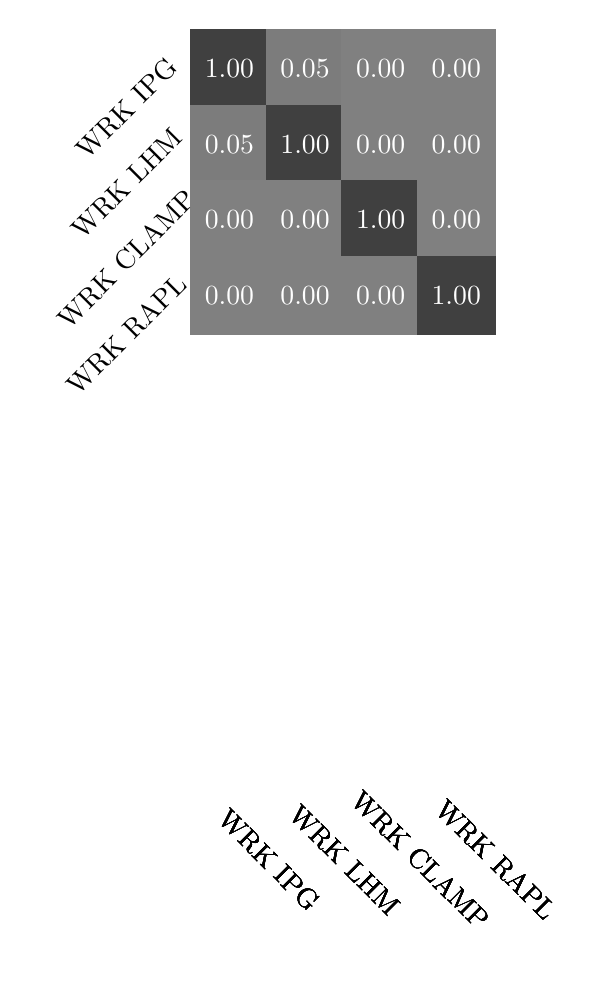
\begin{tikzpicture}[scale=0.6]
      \foreach \y [count=\n] in {{1.00, 0.05, 0.00, 0.00},{0.05, 1.00, 0.00, 0.00},{0.00, 0.00, 1.00, 0.00},{0.00, 0.00, 0.00, 1.00},} {
      % column labels
      \foreach \a [count=\n] in {WRK IPG,WRK LHM,WRK CLAMP,WRK RAPL} {
        \node[minimum size=10mm, xshift=0.5cm, rotate=-45] at (\n*1.6, -18.35) {\a};
      }
      % heatmap tiles
      \foreach \x [count=\m] in \y {
        \pgfmathsetmacro{\xa }{(\x + 1) / 2 * 100}
        \node[fill=darkgray!\xa!lightgray, minimum size=10mm, text=white, font={\normalsize}] at (\m*1.6,-\n*1.6) {\x};
      }
    }
      % row labels
      \foreach \a [count=\i] in {WRK IPG,WRK LHM,WRK CLAMP,WRK RAPL} {
        \node[minimum size=10mm, xshift=-0.35cm, yshift=-0.5cm, rotate=45] at (0,-\i*1.6) {\a};
      }
    \end{tikzpicture}
    \label{tab:HeatFannkuchRedux2}
\end{figure}

\paragraph{Results:} The results from the Mann-Whitney U test can be seen here in \cref{tab:HeatFannkuchRedux2}, and the results from the rest of the test cases can be found in \cref{app:stat2}. In \cref{tab:HeatFannkuchRedux2} the results from the test case FannkuchRedux can be seen, where a similar tendency to the first experiment can be observed. This tendency is that we can reject $H_0$ in most cases. When comparing this analysis to the one conducted in the first experiment, we find more cases where we cannot reject $H_0$ in this experiment. This could be a result of fewer measurements compared to the first experiment, meaning outliers has a larger effect.

\subsection{Correlation}\label{subsec:correlation2}
In this section, the correlation between the different measuring instruments will be conducted for the second experiment. The Kendall Tau coefficients\cite{kendall1938new} will again be used as it was in \cref{subsec:correlation1}

\paragraph{Expectations:} The expectations for the correlations when the C-states are disabled will either be a similar or higher correlation. If the similarity increases, it would be expected to be because the uncertainty of the C-states has been removed.

\begin{figure}
    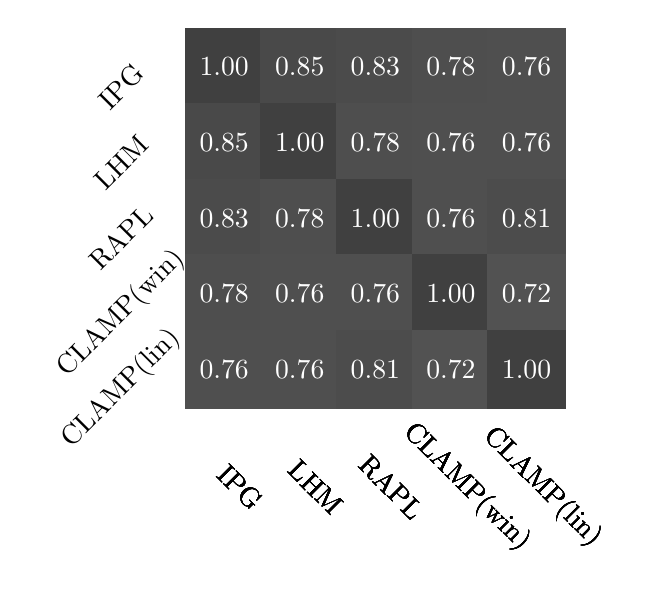
\begin{tikzpicture}[scale=0.6]
      \foreach \y [count=\n] in {{1.00, 0.85, 0.83, 0.78, 0.76},{0.85, 1.00, 0.78, 0.76, 0.76},{0.83, 0.78, 1.00, 0.76, 0.81},{0.78, 0.76, 0.76, 1.00, 0.72},{0.76, 0.76, 0.81, 0.72, 1.00},} {
      % column labels
      \foreach \a [count=\n] in {IPG,LHM,RAPL,CLAMP(win),CLAMP(lin)} {
        \node[minimum size=10mm, xshift=0.2cm, rotate=-45] at (\n*1.6, -10.5) {\a};
      }
      % heatmap tiles
      \foreach \x [count=\m] in \y {
        \pgfmathsetmacro{\xa }{(\x + 1) / 2 * 100}
        \node[fill=darkgray!\xa!lightgray, minimum size=10mm, text=white, font={\normalsize}] at (\m*1.6,-\n*1.6) {\x};
      }
    }
      % row labels
      \foreach \a [count=\i] in {IPG,LHM,RAPL,CLAMP(win),CLAMP(lin)} {
        \node[minimum size=10mm, xshift=-0.35cm, yshift=-0.25cm, rotate=45] at (0,-\i*1.6) {\a};
      }
    \end{tikzpicture}
    \label{tab:correlationWork2}
\end{figure}

\paragraph{Results:} The calculated Correlations for this experiment can be seen in \cref{tab:correlationWork2}. These results look very similar to the similarities obtained from the first experiment in \cref{subsec:correlation1}. The average correlation from experiments on the workstation is as follows:

$$\text{AvgCoefEx1} = (0.81+0.80+0.77+0.71+0.80+0.78+0.71+0.77+0.72+0.70)/10 = 0.757$$
$$\text{AvgCoefEx2} = (0.85+0.83+0.78+0.76+0.78+0.76+0.76+0.76+0.81+0.72)/10 = 0.781$$

These coefficients show higher correlations between the different DUTs and their measuring instruments. Now, the coefficients will be analyzed and utilized to answer our research questions. 

\paragraph{RQ2:} When comparing the measuring instruments to each other the average correlation for each instrument can be calculated. These will then be compared with the results from \cref{sec:Stat1}, to see what effect disabling the C-States have had on the measurements.

\begin{itemize}
    \item \textbf{Experiment 1}
    \begin{itemize}
        \item $IPG = 0.772$ %0.81+0.80+0.77+0.71
        \item $LHM = 0.775$ %0.81+0.80+0.78+0.71
        \item $RAPL = 0.725$ %0.80+0.80+0.77+0.72
        \item $CLAMP(win) = 0.755$ %0.77+0.78+0.77+0.70
        \item $CLAMP(lin) = 0.710$ %0.71+0.71+0.72+0.70
    \end{itemize}
    \item \textbf{Experiment 2}
    \begin{itemize}
        \item $IPG = 0.805$ %0.85+0.83+0.78+0.76
        \item $LHM = 0.787$ %0.85+0.78+0.76+0.76
        \item $RAPL = 0.795$%0.83+0.78+0.76+0.81
        \item $CLAMP(win) = 0.755$ %0.78+0.76+0.76+0.72
        \item $CLAMP(lin) = 762$ % 0.76+0.76+0.81+0.72
    \end{itemize}
\end{itemize}

When looking at the average correlation for the measuring instruments across the two experiments, the second experiment generally had larger coefficients than the first experiment, showing a higher correlation for the second experiment. Looking at these numbers using the Guildford scale, it can be seen how the correlation does not increase enough to change evaluation.

\paragraph{RQ3:} When comparing the results across OSs, some differences can be observed when compared to the first experiment. The OS benefitting the most in terms of correlation coefficients when disabling the C-Stats is Linux, as the correlation between RAPL and the other measuring instruments increased. This is mostly dues to an increased correlation between RAPL and the clamp on Linux, which increased from $0.72$ to $0.81$.  Overall it seems that RAPL is the measuring instrument most closely correlated with the hardware measurements while IPG is the most correlated measuring instrument for Windows.





% \begin{table}[]
    \begin{tabular}{||c|c|c|c|c|c||}    \hline
    &\textbf{TestCaseIdle}&\textbf{BinaryTrees}&\textbf{FannkuchRedux}&\textbf{Nbody}&\textbf{Fasta}\\ [0.5ex] \hline
    \hline \textbf{IntelPowerGadget}&0.0&\textbf{0.9103}&\textbf{0.1293}&0.0002&\textbf{0.8291}\\
    \textbf{HardwareMonitor}&0.0213&\textbf{0.1345}&0.0492&\textbf{0.3209}&0.0\\
    \textbf{Clamp Win}&0.0034&0.0023&0.012&\textbf{0.8143}&\textbf{0.5335}\\
    \textbf{RAPL}&\textbf{0.1899}&\textbf{0.5744}&0.0015&\textbf{0.9437}&\textbf{0.0518}\\
    \textbf{Clamp Lin}&\textbf{0.4601}&0.0004&0.0&\textbf{0.1006}&0.0002\\ \hline \end{tabular}
    \caption{P values for the normal distribution for the Workstation in Ex2}\label{tab:NormDist2}
\end{table} 

% As can be seen in \cref{tab:NormDist2}, the data is not normally distributed the data from experiment 2 is generally further away from being normally distributed than the experiment 1. This is not that surprising given that experiment 2 contain less actual runs as these were not needed as found in \cref{subsec:CockUse}. 

% For the MannWhitney U test we would again expect very similar results to the results from experiment one, where the null hypotheses can be rejected in most of the cases.
% The results from the MannWhitney U test can be seen here in \cref{tab:HeatFannkuchRedux2}.
% \begin{figure}
    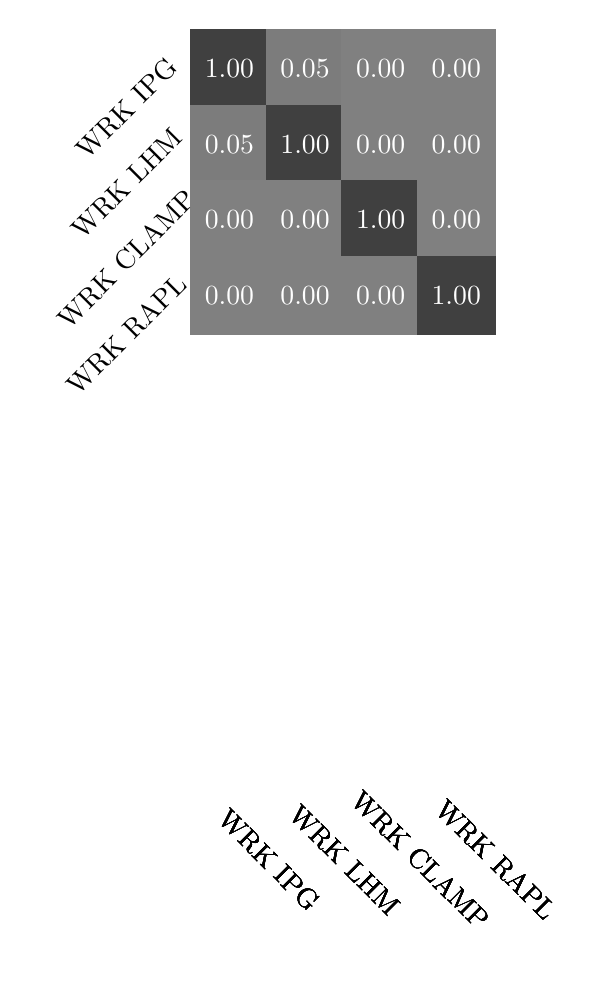
\begin{tikzpicture}[scale=0.6]
      \foreach \y [count=\n] in {{1.00, 0.05, 0.00, 0.00},{0.05, 1.00, 0.00, 0.00},{0.00, 0.00, 1.00, 0.00},{0.00, 0.00, 0.00, 1.00},} {
      % column labels
      \foreach \a [count=\n] in {WRK IPG,WRK LHM,WRK CLAMP,WRK RAPL} {
        \node[minimum size=10mm, xshift=0.5cm, rotate=-45] at (\n*1.6, -18.35) {\a};
      }
      % heatmap tiles
      \foreach \x [count=\m] in \y {
        \pgfmathsetmacro{\xa }{(\x + 1) / 2 * 100}
        \node[fill=darkgray!\xa!lightgray, minimum size=10mm, text=white, font={\normalsize}] at (\m*1.6,-\n*1.6) {\x};
      }
    }
      % row labels
      \foreach \a [count=\i] in {WRK IPG,WRK LHM,WRK CLAMP,WRK RAPL} {
        \node[minimum size=10mm, xshift=-0.35cm, yshift=-0.5cm, rotate=45] at (0,-\i*1.6) {\a};
      }
    \end{tikzpicture}
    \label{tab:HeatFannkuchRedux2}
\end{figure}
% The shown table in \cref{tab:HeatFannkuchRedux2}, is again from the FannkuchRedux Test Case as in \cref{subsec:Stat1}. Again we see a similar tendency in that for most cases we can reject $H_0$, but for experiment 2 there are a few more cases where we cannot reject $H_0$. Once possible reason why that might be the case is that there are fewer samples in experiment 2 so outlier have a larger effect on the Ex1Statistics.

% Finally for the Correlations between the measuring instruments, the expectations for the correlations in Experiment 2 is that they are either are a bit more correlated since the uncertainty's of the C-Stats have been removed, or that i will remain nearly exactly the same. The calculated Correlations for experiments 2 can be seen in \cref{tab:correlationWork2}.
% \begin{figure}
    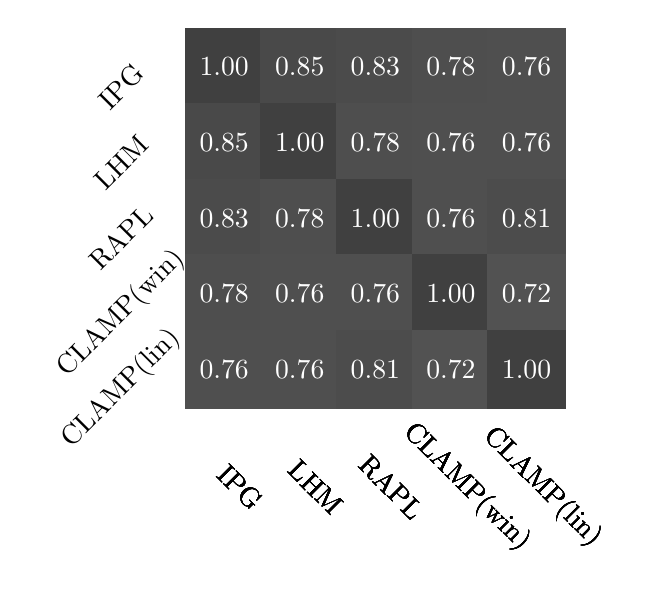
\begin{tikzpicture}[scale=0.6]
      \foreach \y [count=\n] in {{1.00, 0.85, 0.83, 0.78, 0.76},{0.85, 1.00, 0.78, 0.76, 0.76},{0.83, 0.78, 1.00, 0.76, 0.81},{0.78, 0.76, 0.76, 1.00, 0.72},{0.76, 0.76, 0.81, 0.72, 1.00},} {
      % column labels
      \foreach \a [count=\n] in {IPG,LHM,RAPL,CLAMP(win),CLAMP(lin)} {
        \node[minimum size=10mm, xshift=0.2cm, rotate=-45] at (\n*1.6, -10.5) {\a};
      }
      % heatmap tiles
      \foreach \x [count=\m] in \y {
        \pgfmathsetmacro{\xa }{(\x + 1) / 2 * 100}
        \node[fill=darkgray!\xa!lightgray, minimum size=10mm, text=white, font={\normalsize}] at (\m*1.6,-\n*1.6) {\x};
      }
    }
      % row labels
      \foreach \a [count=\i] in {IPG,LHM,RAPL,CLAMP(win),CLAMP(lin)} {
        \node[minimum size=10mm, xshift=-0.35cm, yshift=-0.25cm, rotate=45] at (0,-\i*1.6) {\a};
      }
    \end{tikzpicture}
    \label{tab:correlationWork2}
\end{figure}
% At an first these results look very similar to the once from experiment 1, but to verify these number more in depth we can compare the averages of the correlations as before.


% This slight increase in overall correlation matches up with our expectations as the added consistency in the experiments should help reduce inconsistencies. Generally the correlations are higher in experiment 2, but the correlation does fall in certain cases, these cases will be looked at a bit here.

% The first case is the $RAPL|CLAMP(win)$ which used to in experiment one to have a coefficients of $0.77$, but in Experiment 2 as $0.76$, while this is only a marginal decrease it could be caused by the fact that one measures linux and the other windows. Another one is $LHM|RAPL$ which went from $0.80$ to $0.78$ these measurements are again done on separate OSs. 

% So the divide between linux and windows seems to have gotten larger.   









